\documentclass[11pt]{article}

\usepackage[margin=1in]{geometry}
\usepackage{amsmath,amssymb}
\usepackage{graphicx}
\usepackage{booktabs}
\usepackage{hyperref}

\graphicspath{{../output/}}
% Generated by src/q2b.py -- do not edit by hand.
\newcommand{\QtwobCorr}{0.355}
\newcommand{\QtwobT}{1190}
 % \QtwobCorr, \QtwobT (generated by src/q2b.py)

\title{BUSFIN 8200: Asset Pricing Foundations\\Problem Set 2}
\author{} % TODO (student): name
\date{\today}

\begin{document}
\maketitle

\section*{Question 1}
% TODO (student)

\section*{Question 2}

\subsection*{2a)}
% Produced by src/q2a.py (spec: spec/q2a.md). Estimates: output/q2a_sdf_coefficients.csv.

% TODO (student): describe the pattern you observe in the scatterplot.

% TODO (student): explain why this pattern emerges.

\begin{figure}[htbp]
  \centering
  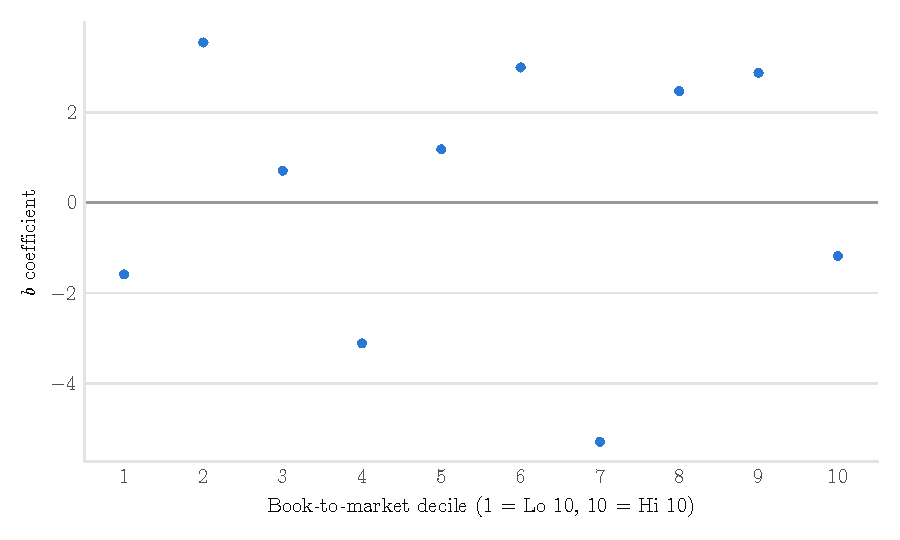
\includegraphics[width=0.85\textwidth]{q2a_b_scatter.pdf}
  \caption{Coefficients $b$ of the SDF $M^*_t = a - b'xR_t$ that prices the monthly excess
    returns of the 10 value-weighted book-to-market decile portfolios (July 1927 to August
    2026), under the normalization $\widehat{\mathbb{E}}[M^*] = 1$. Excess returns are in
    decimal units.}
  \label{fig:q2a_b}
\end{figure}

\subsection*{2b)}
% Produced by src/q2b.py (spec: spec/q2b.md). Estimates: output/q2b_sdf_coefficients.csv.

% TODO (student): describe the pattern you observe in the scatterplot.

% TODO (student): explain why this pattern emerges.

% Correlation between M*_t from 2a) and 2b). Value generated by src/q2b.py
% (output/q2b_sdf_correlation.tex); reporting sentence drafted by AI (AI_INTERACTIONS.md).
The sample (Pearson) correlation between the monthly SDF series $M^*_{\mathrm{BM},t}$
estimated in 2a) and $M^*_{\mathrm{MOM},t}$ estimated in 2b), over July 1927 to August 2026
($T = \QtwobT$ months), is
\[
  \widehat{\mathrm{Corr}}\left(M^*_{\mathrm{BM},t},\, M^*_{\mathrm{MOM},t}\right) = \QtwobCorr .
\]

% TODO (student): interpret this correlation in economic terms.

\begin{figure}[htbp]
  \centering
  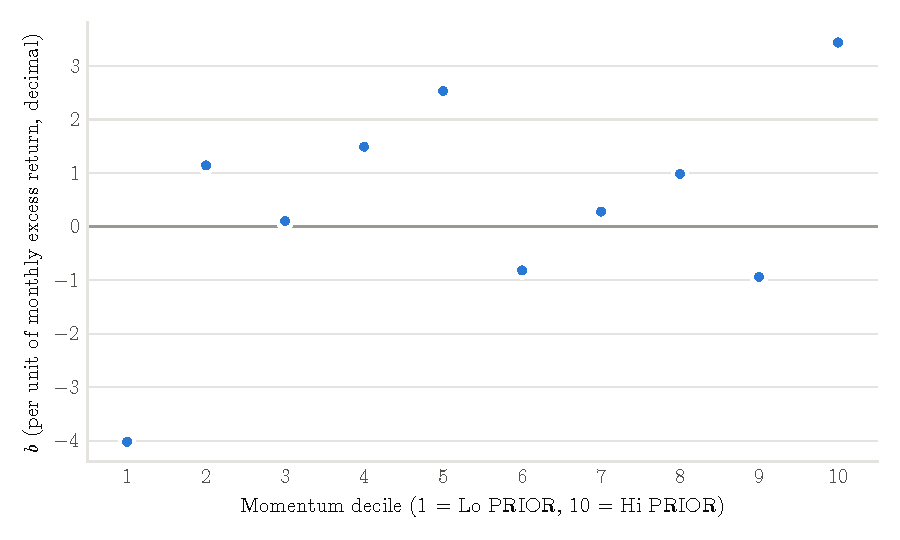
\includegraphics[width=0.85\textwidth]{q2b_b_scatter.pdf}
  \caption{Coefficients $b$ of the SDF $M^*_t = a - b'xR_t$ that prices the monthly excess
    returns of the 10 value-weighted momentum (prior 12--2 month return) decile portfolios
    (July 1927 to August 2026), under the normalization $\widehat{\mathbb{E}}[M^*] = 1$.
    Excess returns are in decimal units.}
  \label{fig:q2b_b}
\end{figure}

\section*{Question 3}
% TODO (student)

\section*{Question 4}
% TODO (student)

\end{document}
